%%%%%%%%%%%%%%%%%%%%%%%%%%%%%%%%%%%%%%%%%%%%%%%%%%%%%%%%%%%%%%%%%%% 
%                                                                 %
%                            CHAPTER                              %
%                                                                 %
%%%%%%%%%%%%%%%%%%%%%%%%%%%%%%%%%%%%%%%%%%%%%%%%%%%%%%%%%%%%%%%%%%% 

\chapter{Introduction}

\section{Problem description}

    The steel industry is a big industry in the world and provides 2.5 million jobs across Europe according to the European commission. Due to high labor costs in western Europe and more specific in Belgium here labour costs are about 40\% above the average of labour costs in Europe. For this reason production and manufacturing costs should lower to be able to compete with other companies around the world. 
    
Metal carving is done by using a rotary holder which spins over the metal work piece and carves away material. This rotary holder keeps inserts as seen in Figure \ref{fig:gen:insertholder}. They are kept in place with a screw for easy removal and replacement. The inserts are made of different carbides mostly Wolfram carbide and get a coating on the outer layer to provide extra strength and more capabilities to cut different materials. The cutting part on the corner of the insert will wear when the work piece is carved and will result in a bad finish on the actual product if it is not replaced in time. 
    
\begin{figure}[hbtp]
\centering
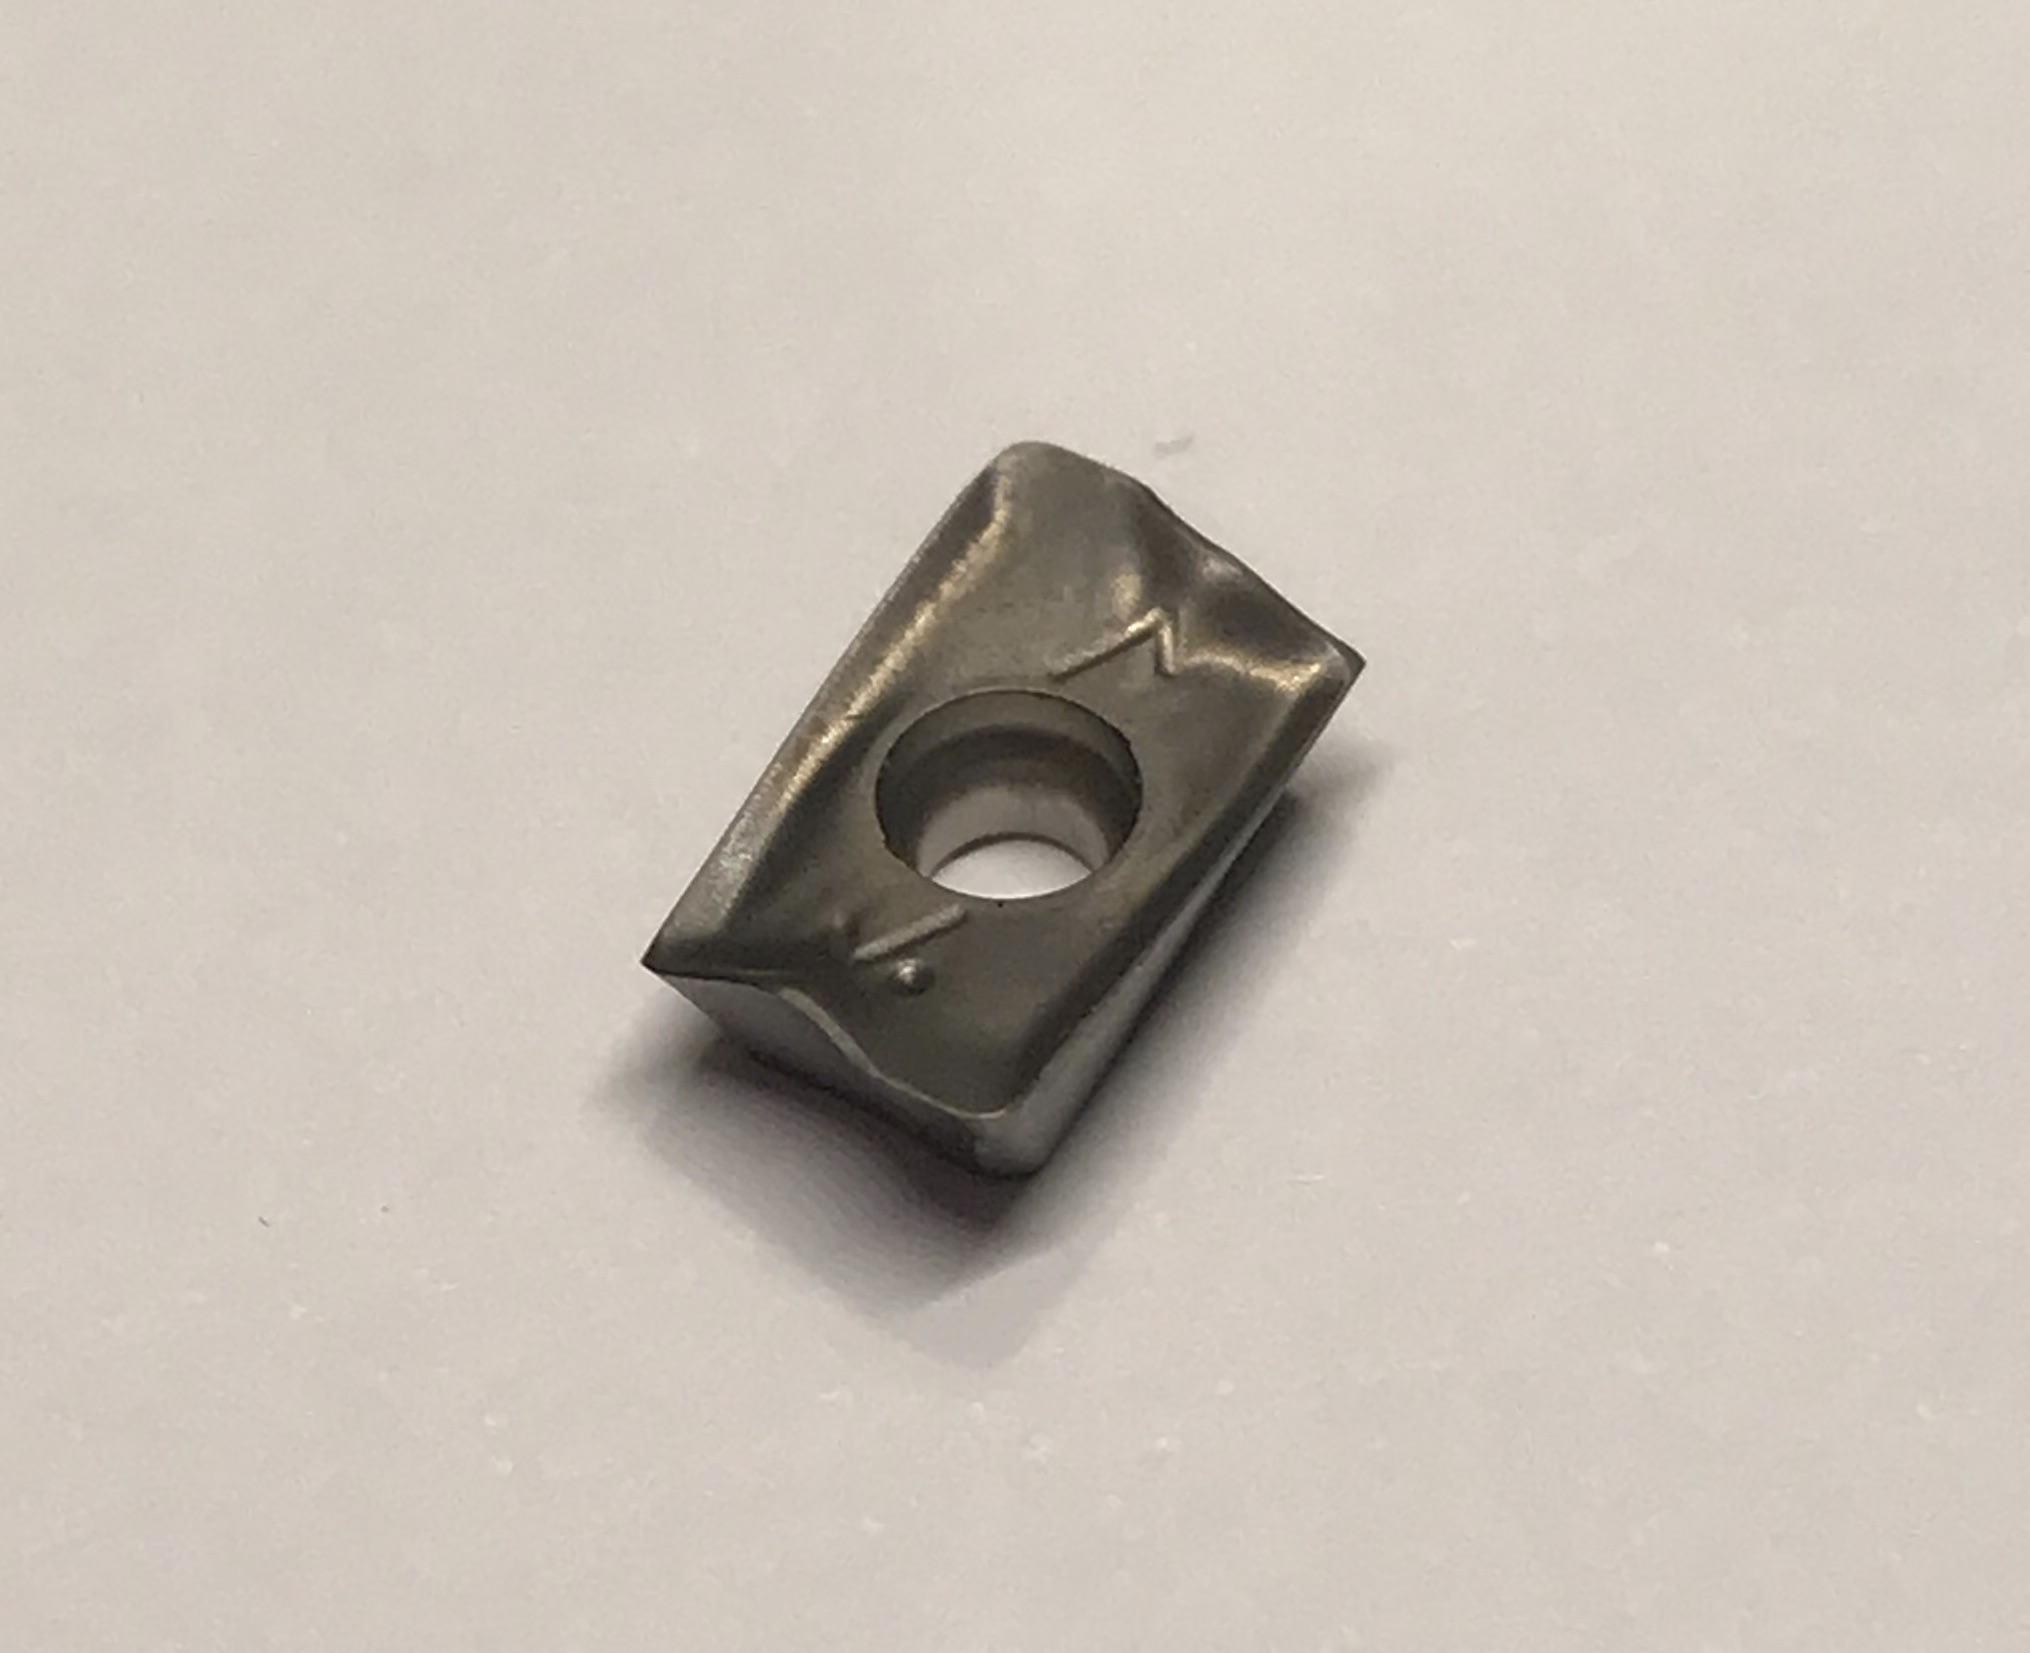
\includegraphics[scale=0.04]{fig/algemeen/plaatjes/plaatje/plaatje_top_corner.jpeg}
\label{fig:gen:insert1x1}
\caption{Picture of an insert on 1cm by 1cm grid}
\end{figure}

\begin{figure}[hbtp]
\centering
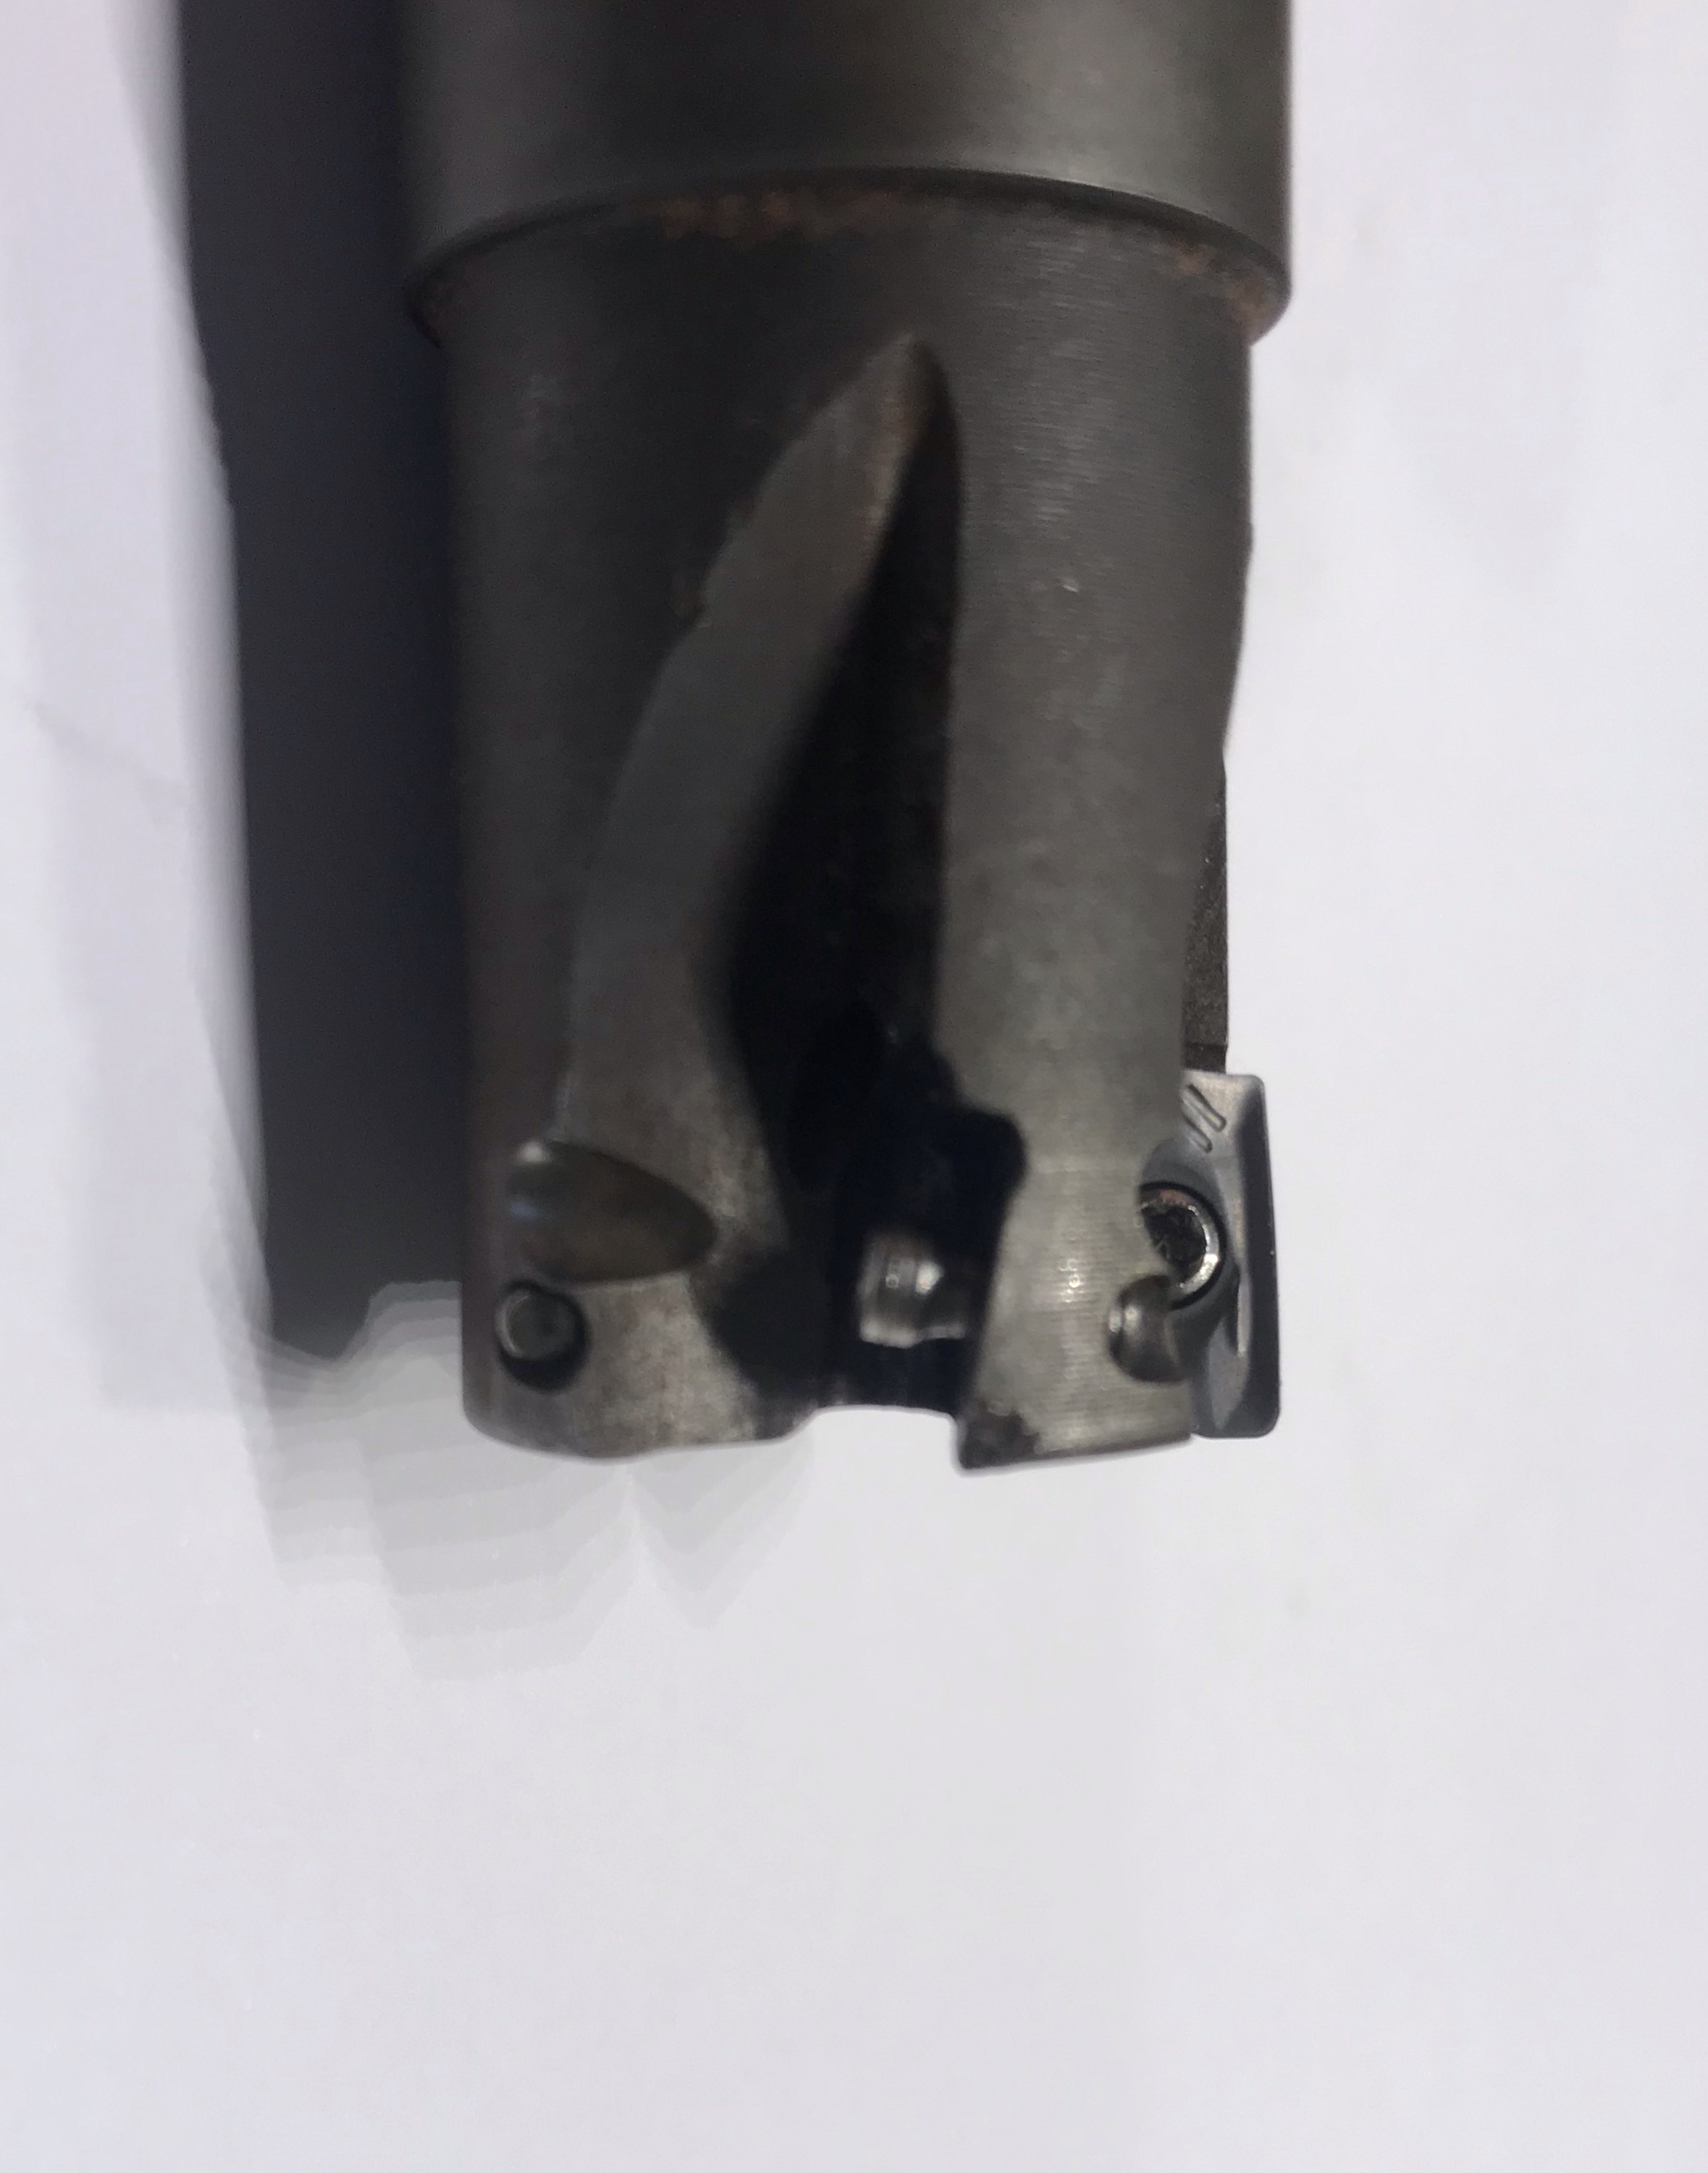
\includegraphics[scale=0.1]{fig/algemeen/plaatjes/houder/rotary_holder.jpeg}
\caption{Rotary holder with one insert in place.}
 \label{fig:gen:insertholder}
\end{figure}


   
    
    For the replacement of the inserts there are two policies used today:
    \begin{enumerate}
        \item Check the inserts when a work piece is finished.
        \item Replacing all inserts on set time intervals (e.g. every 30 minutes).
    \end{enumerate}
     Although option number one will optimize the lifespan of the inserts, it is very time consuming and labor intensive. Option number two is less labor intensive and thus less time consuming but will produce a lot of waste in those inserts. Having safety levels there will be a lot of inserts thrown away even when they are still usable.
     
     Insert more context on the equipment
     
insert overview of the whole paper